\section{Data Access}
\label{sec:databases}

%%%%%%%---- BEGIN ----  ----%%%%%%
\begin{frame}
  \frametitle{Databases and Data Aggregators}

  \begin{columns}[T]

      \begin{column}{.3\textwidth}
        \only<1>{%
          \vspace{0.5em}
\includegraphics[width=.8\textwidth]{logo_cds}\\
          \vspace{0.5em}
\includegraphics[width=.8\textwidth]{logo_pds}\\
          % \vspace{0.5em}
\includegraphics[width=.8\textwidth]{logo_mp3c}\\
          % \vspace{0.5em}
\includegraphics[width=.8\textwidth]{logo_ssodnet}\\
        }%
        \only<2->{%
          \vspace{0.5em}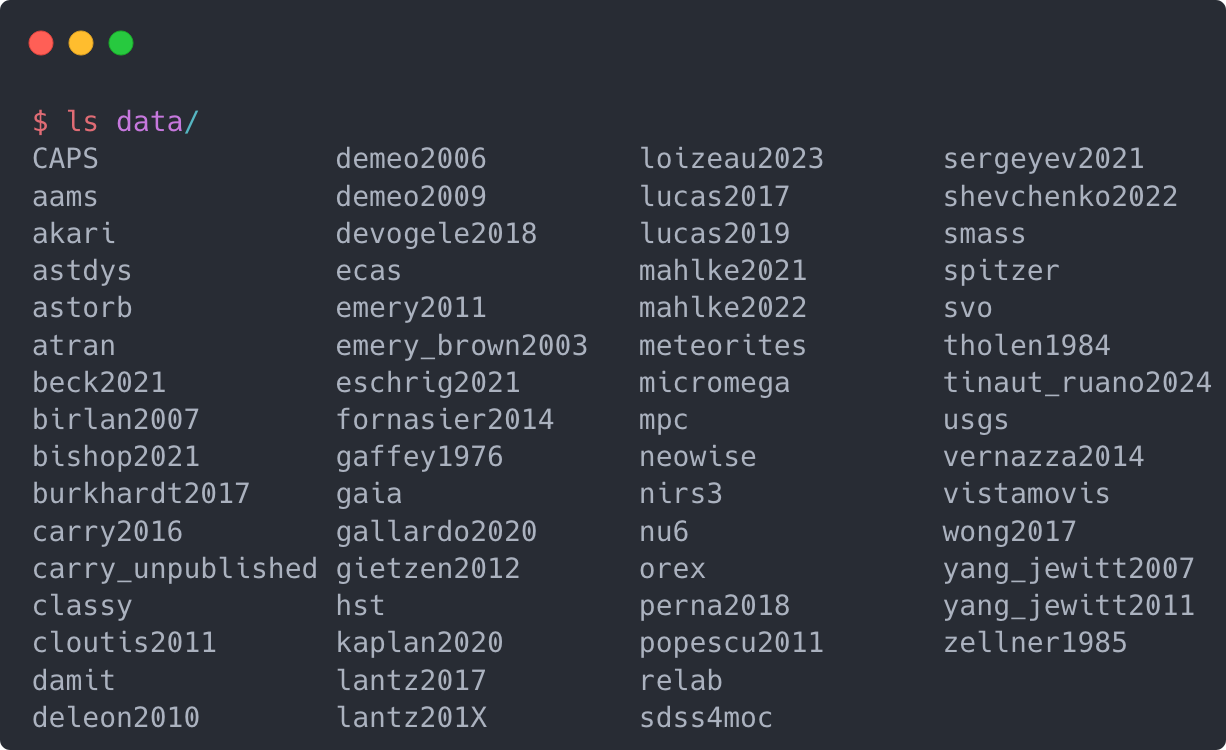
\includegraphics[width=.8\textwidth]{data_dir}\\
          \vspace{0.5em}
\includegraphics[width=.8\textwidth]{logo_astorb}\\
          \vspace{0.5em}
\includegraphics[width=.8\textwidth]{logo_mp3c}\\
          \vspace{0.5em}
\includegraphics[width=.8\textwidth]{logo_ssodnet}\\
        }%
      \end{column}


    \begin{column}{.7\textwidth}
      \begin{overlayarea}{\textwidth}{\textheight}
          \vspace{1em}
          We all need data, we all generate data.\\
          \vspace{1em}
          \begin{itemize}[<.->]
            \item \emph{\bf Databases}
              \begin{itemize}[<.->]
                \item[$\circ$] Websites, CDS, on request
                \item[$\circ$] Mostly static, single bibliographic reference
                \item[$\circ$] Mixture of formats
              \end{itemize}

            \only<2->{%
            \vspace{0.5em}
            \item \emph{\bf Data Aggregators}
              \begin{itemize}[<.->]
                \item[$\circ$] Collection of data \emph{with processing}
                \item[$\circ$] Dynamic, large number of bibliography references
                \item[$\circ$] Uniform output
              \end{itemize}
            }%
          \end{itemize}

          \only<3->{%
          \vspace{0.5em}
          Data aggregation takes effort but saves time and energy.
          }%
      \end{overlayarea}
    \end{column}

  \end{columns}

\end{frame}

\begin{frame}[t]
  \frametitle{Data Aggregators}
  {\scriptsize
  \begin{table}[t]
    \begin{tabular}{llll}
      \textsc{Name} & \textsc{Objects} & \textsc{Parameters} & \textsc{URL} \bigskip\\
      ECOCEL & Asteroids & Physical, Orbital &  \tiny \url{http://www.ecocel-database.com/}\smallskip\\
      \alt<2>{\emph{JPL SBDB}}{JPL SBDB} & Asteroids, Comets & Physical, Orbital & \tiny \url{https://ssd.jpl.nasa.gov/tools/sbdb_lookup.html}\smallskip\\
      \alt<2>{\emph{Lowell}}{Lowell} & Asteroids & Physical, Orbital &  \tiny\url{https://asteroid.lowell.edu/astinfo/}\smallskip\\
      \alt<2>{\emph{MP3C}}{MP3C} & Asteroids & Physical, Orbital &  \tiny\url{https://mp3c.oca.eu/}\smallskip\\
      NEOExchange & Near-Earth Objects & Orbital &  \tiny\url{https://neoexchange.lco.global/}\smallskip\\
      SiMDA & Asteroids, Comets & Size, Mass, Density & \tiny \url{https://astro.kretlow.de/simda/}\smallskip\\
      \alt<2>{\emph{SsODNet}}{SsODNet} & Asteroids & Physical, Orbital & \tiny \url{https://ssp.imcce.fr/forms/ssocard}\smallskip\\
    \end{tabular}
  \end{table}
  }
    % Comets -> little tools as well -> SsODNet
\end{frame}

\begin{frame}[t]{Demo}
  The next slides show an outline of the demoed material.
\end{frame}

\begin{frame}[t]{Demo}
  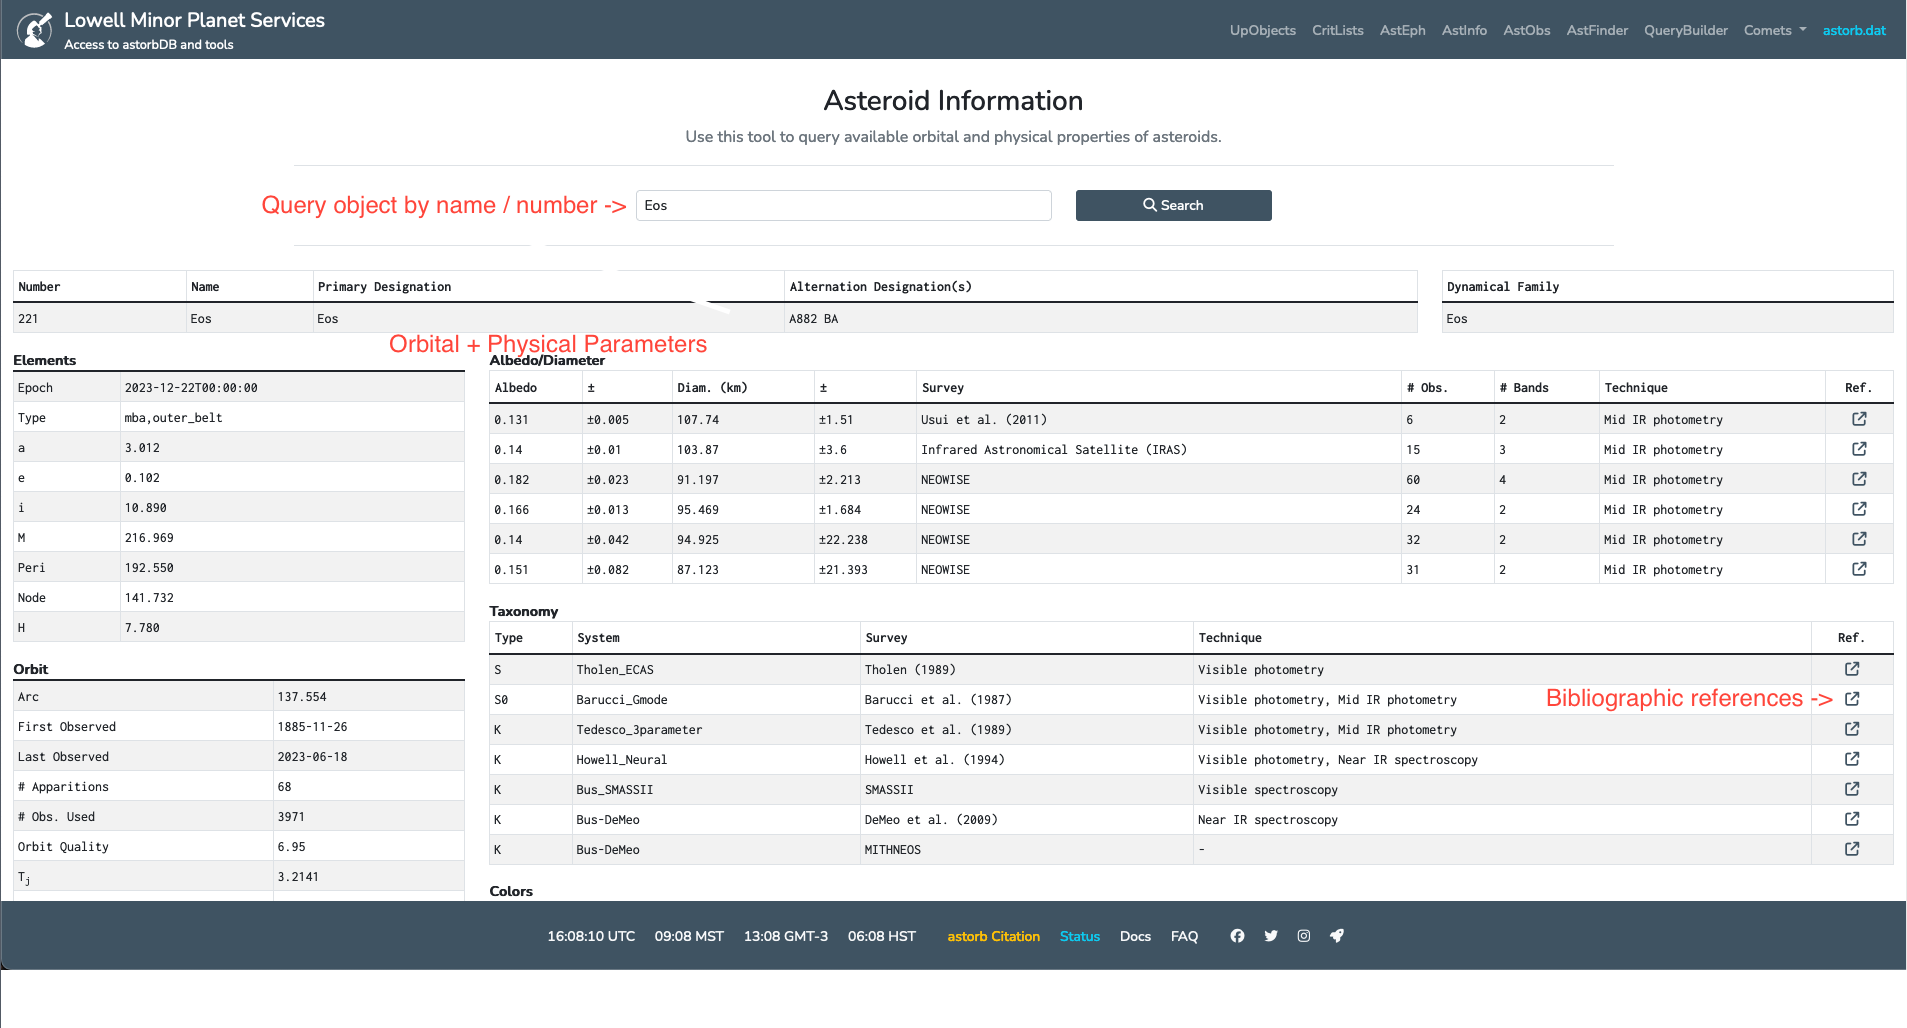
\includegraphics[width=0.9\textwidth]{gfx/demo_lowell.png}
  \url{https://asteroid.lowell.edu/}
\end{frame}

\begin{frame}[t]{Demo}
  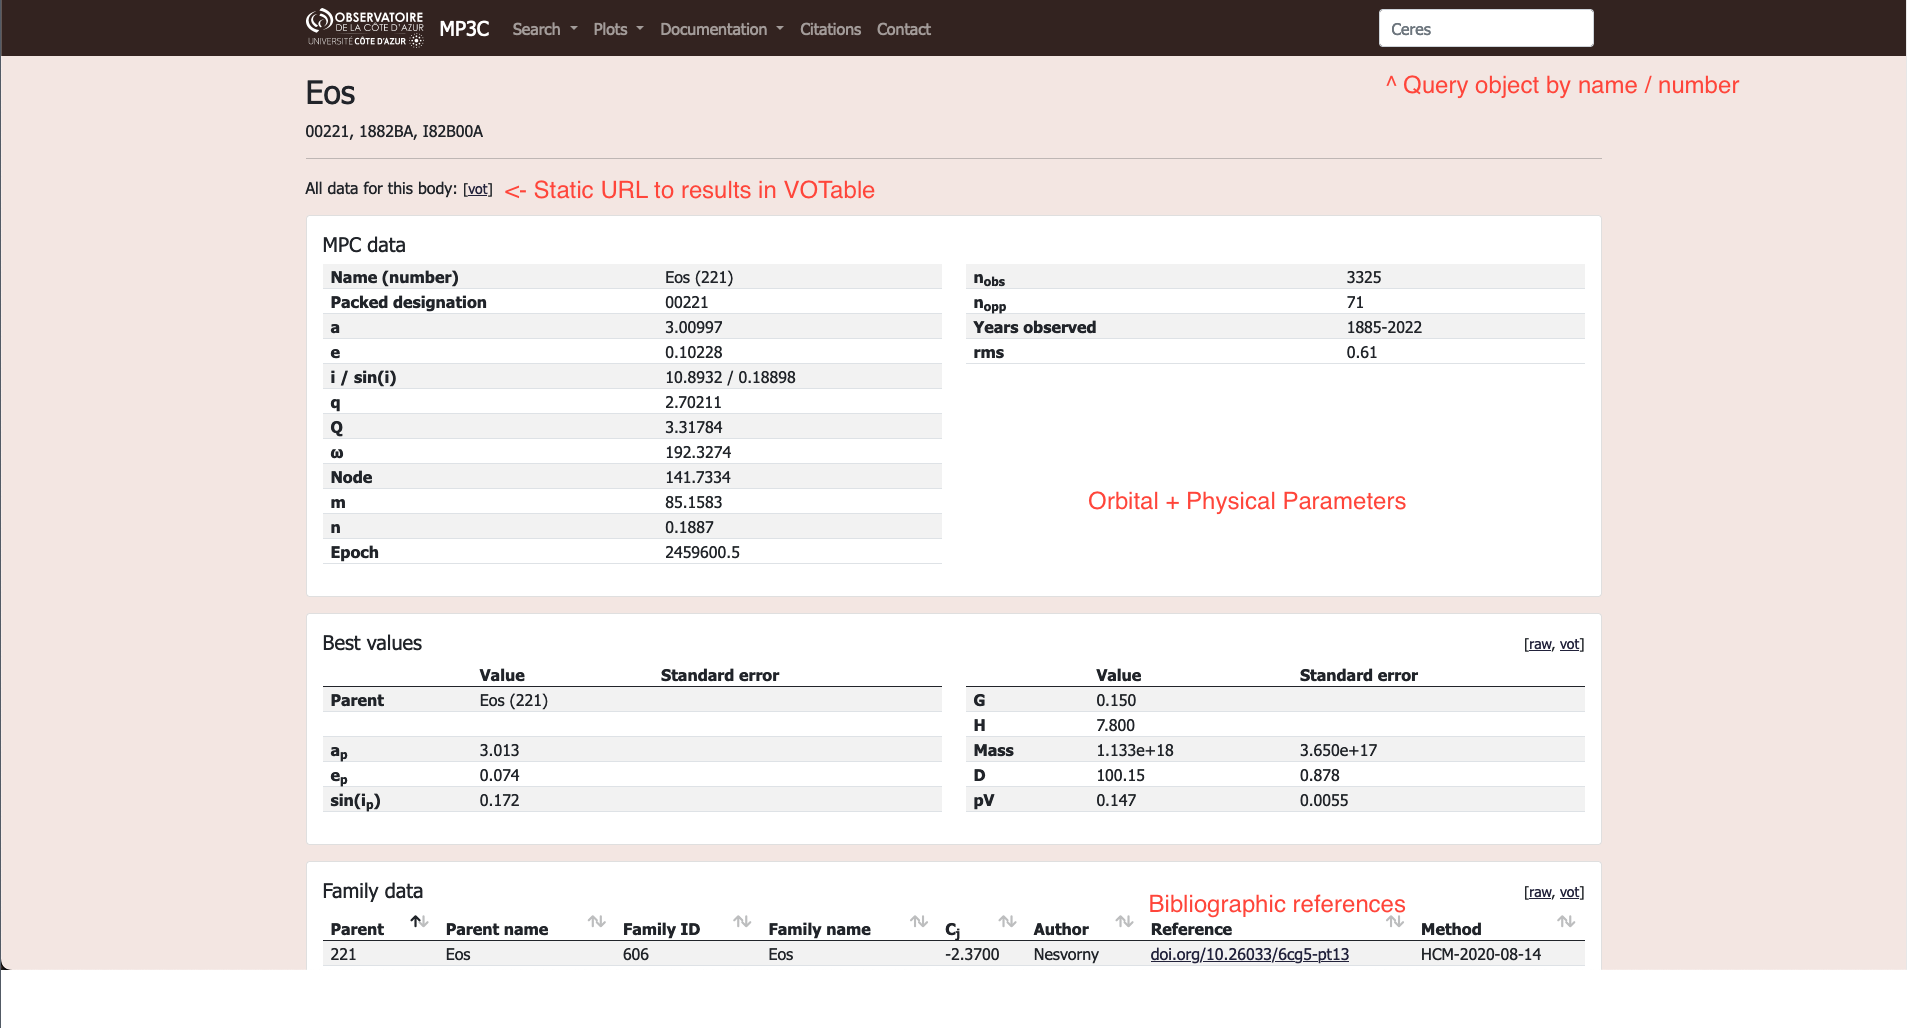
\includegraphics[width=0.9\textwidth]{gfx/demo_mp3c.png}
  \url{https://mp3c.oca.eu/}
\end{frame}

\begin{frame}[t]{Demo}
  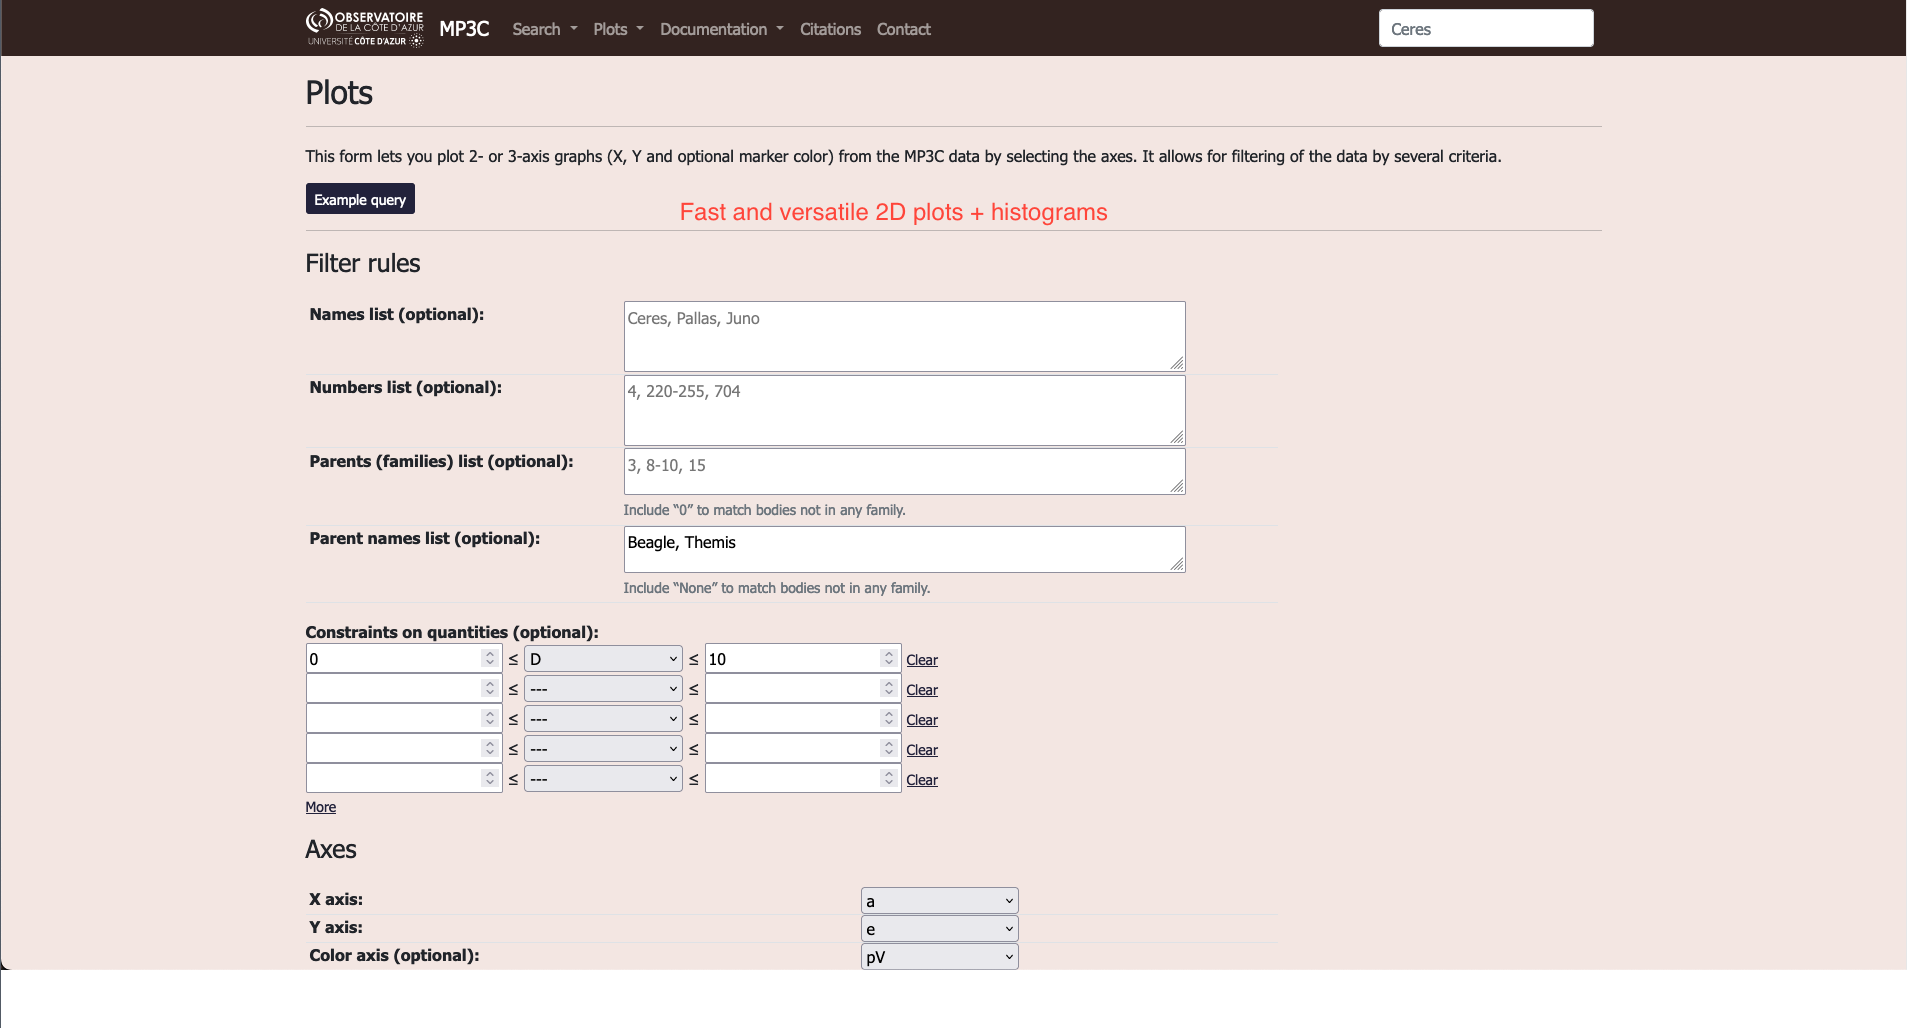
\includegraphics[width=0.9\textwidth]{gfx/demo_mp3c_2.png}
  \url{https://mp3c.oca.eu/xyc-plot/}
\end{frame}

\begin{frame}[t]{Demo}
  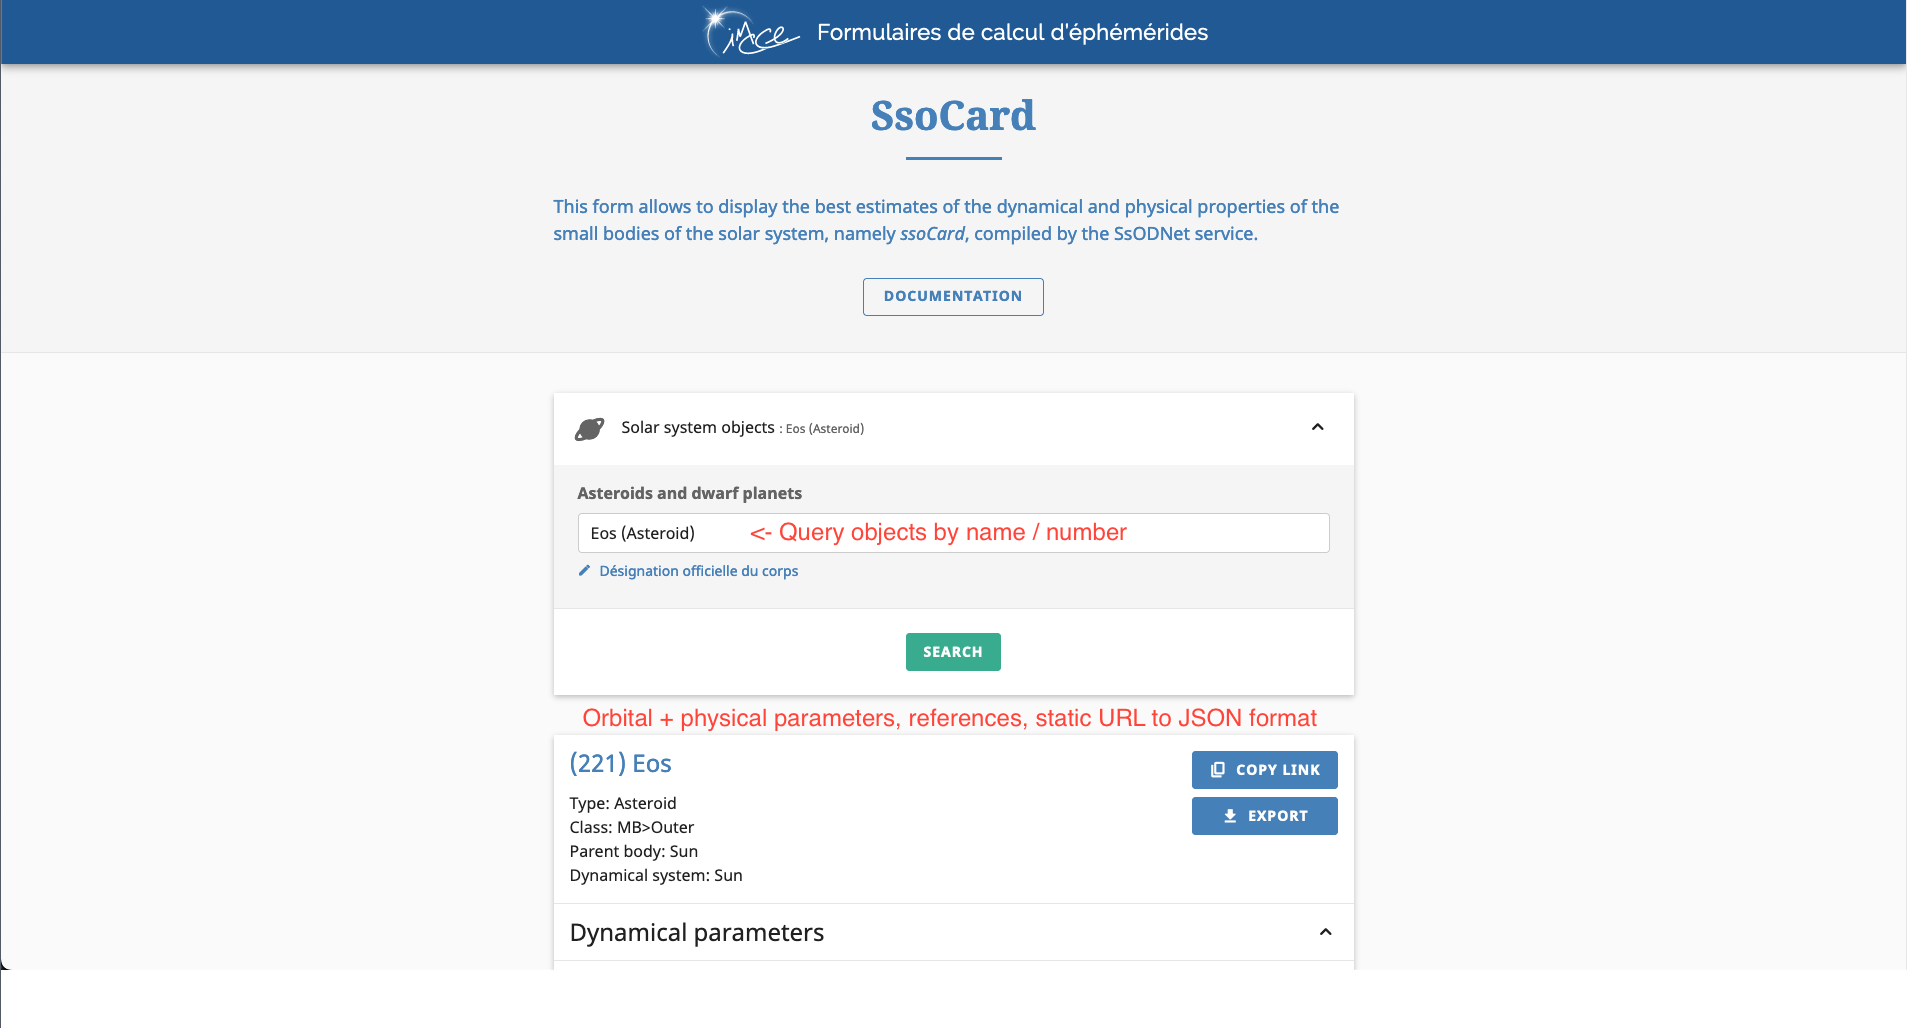
\includegraphics[width=0.9\textwidth]{gfx/demo_ssocard.png}
  \url{https://ssp.imcce.fr/forms/ssocard}
\end{frame}

\begin{frame}[t]{Demo}
  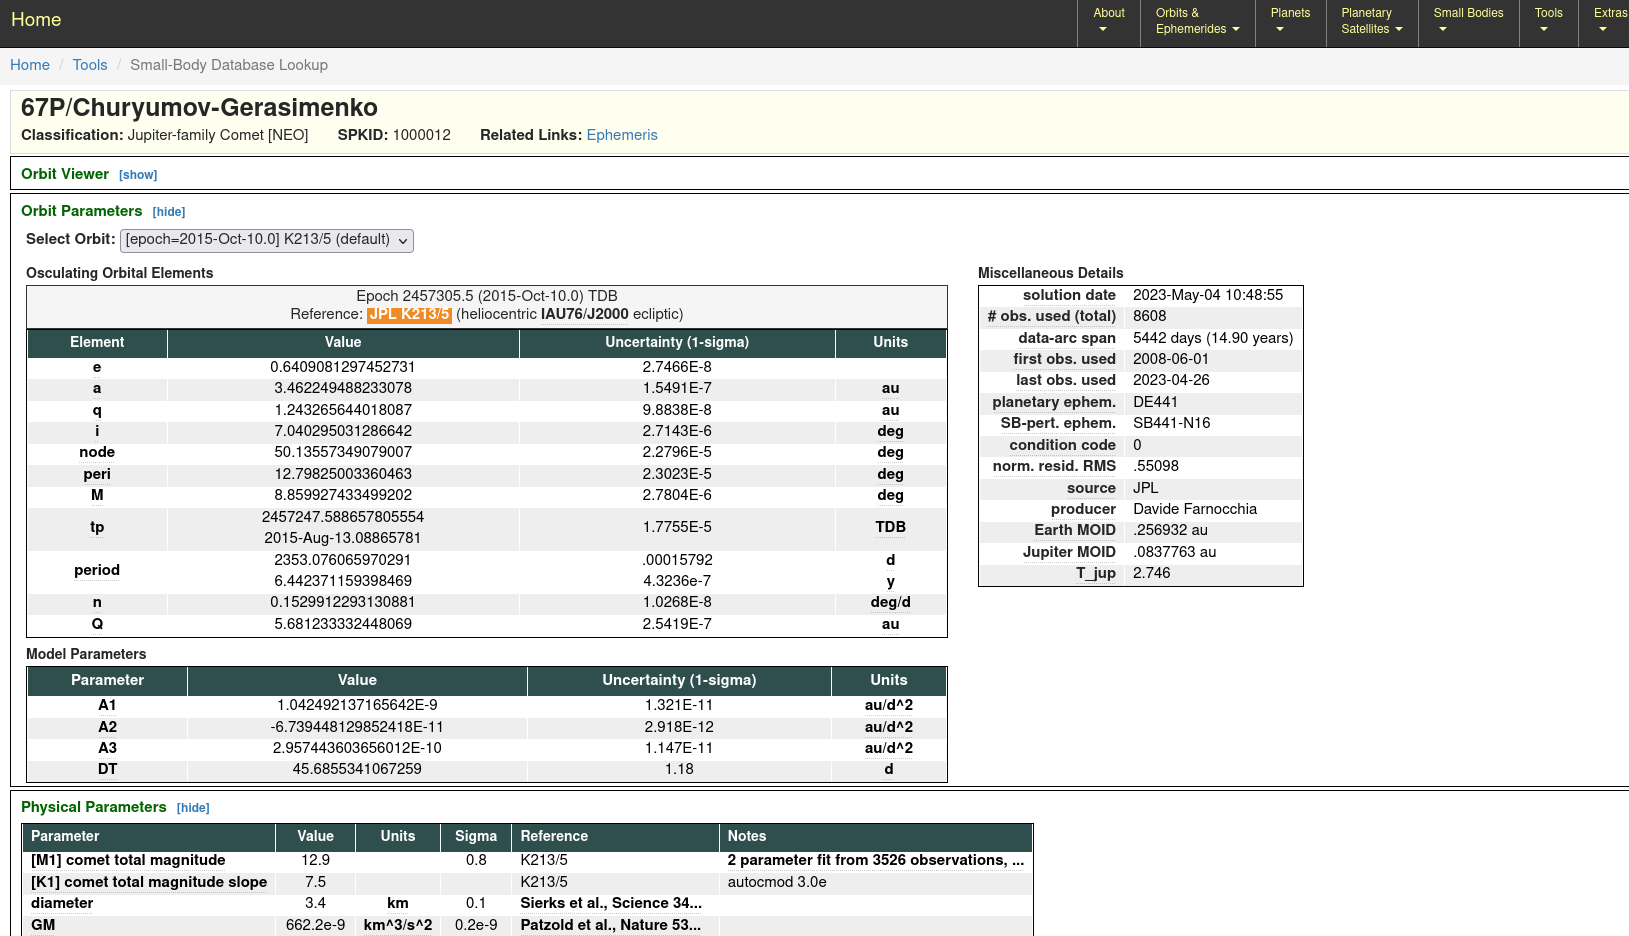
\includegraphics[width=0.8\textwidth]{gfx/demo_jpl.png}
  \url{https://ssd.jpl.nasa.gov/tools/sbdb_lookup.html}
\end{frame}

% \begin{frame}[t]{Data Aggregators}
%     And the meteorites?
%     \smallskip
%     \begin{itemize}
%       \item Meteoritical Bulletin {\tiny\url{https://www.lpi.usra.edu/meteor/}}
%         \begin{itemize}
%           \item Name, classification, fall/find
%           \item Meteorite Name Checking Utility {\tiny\url{https://www.lpi.usra.edu/meteor/metbullcheck.php}}
%         \end{itemize}
%         \vspace{0.5em}
%       \item Antarctic Meteorite Classification Database {\tiny\url{https://curator.jsc.nasa.gov/antmet/}}
%         \begin{itemize}
%           \item[\circ] Has an API :-)
%           \item[\circ] Only records antarctic meteorites :-(
%         \end{itemize}
%     \end{itemize}
%
%     \only<2->{
%       \bigskip
%       Need for a meteorite database + API!
%     }
% \end{frame}

\begin{frame}[t]{The N-Body Problem}

\begin{columns}[T]

      \begin{column}{.3\textwidth}
        \vspace{0.5em}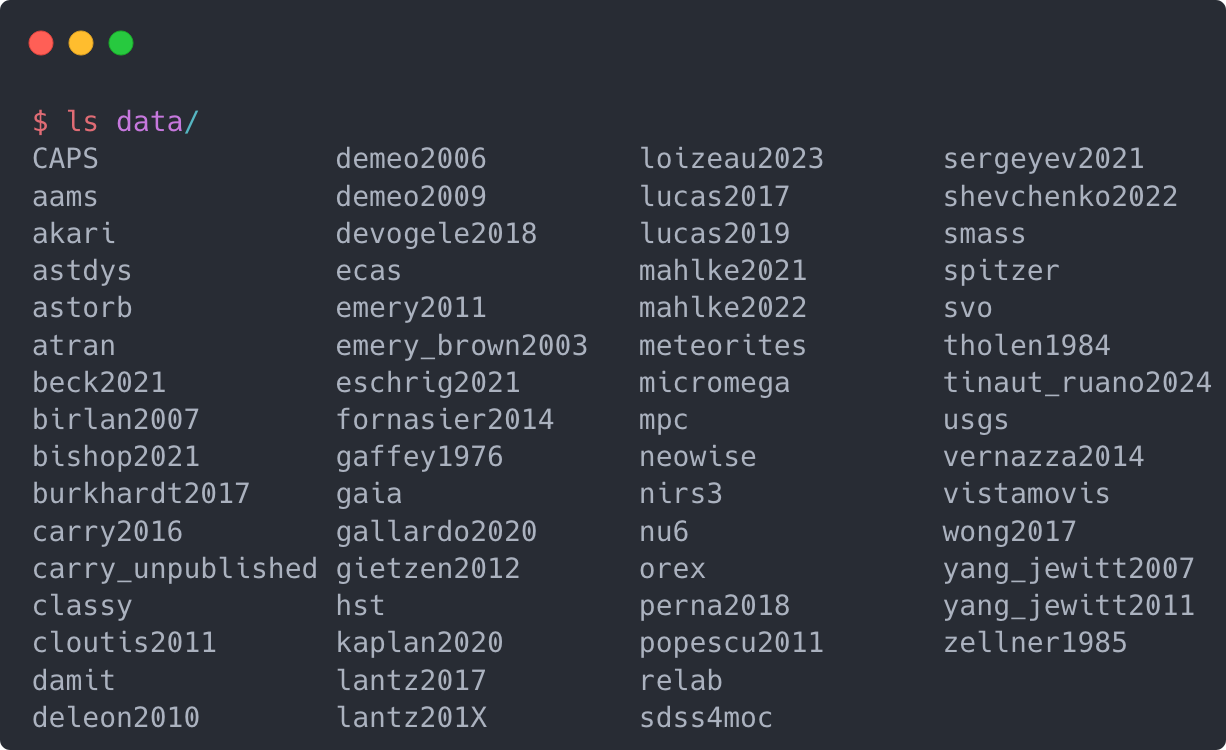
\includegraphics[width=.8\textwidth]{data_dir}\\
        \vspace{0.5em}
\includegraphics[width=.8\textwidth]{logo_astorb}\\
        \vspace{0.5em}
\includegraphics[width=.8\textwidth]{logo_mp3c}\\
        \vspace{0.5em}
\includegraphics[width=.8\textwidth]{logo_ssodnet}\\
      \end{column}

    \begin{column}{.7\textwidth}
      \begin{overlayarea}{\textwidth}{\textheight}

        %
        % We access the same data for many objects multiple times.
        \begin{itemize}[<.->]
          \item \emph{\bf Graphical User Interfaces do not scale}
            \begin{itemize}[<.->]
              \item[$\circ$] Many bodies \textrightarrow Many clicks
              \item[$\circ$] Repeated queries to update data
              \item[$\circ$] Bibliography management
            \end{itemize}
        \end{itemize}
          \textrightarrow~Data aggregators need programmatic APIs

      \vspace{1.0em}
        \begin{itemize}[<.->]
          \item \emph{\bf Different degrees of simplification}
            \begin{itemize}[<.->]
              \item[$\circ$] Static URLs pointing to text files
              \item[$\circ$] Common service such as the \textit{Table Access Protocol}
              \item[$\circ$] Secondary client such as \texttt{python} packages
            \end{itemize}
        \end{itemize}
      \vspace{0.5em}
        % \begin{itemize}[<.->]
        %   \item[\textrightarrow] \emph{\bf We need to know how to use them}
        %     \begin{itemize}[<.->]
        %       \item[$\circ$] Python: API call versus object-oriented programming
        %       \item[$\circ$] Simplify your day-to-day with good code
        %     \end{itemize}
        % \end{itemize}
      \end{overlayarea}
    \end{column}
  \end{columns}

\end{frame}

\begin{frame}[t]{Tutorial}
  [20min] Tutorial notebook on data access
\end{frame}
%%%%%%%----  END  ----  ----%%%%%%
